\chapter{Introduction}

Automatically generating high quality translations for foreign texts remains a central challenge for Natural Language Processing research.
Recent advances in Statistical Machine Translation (SMT) has enabled these technologies to move out of research labs an become viable commercial products and ubiquitous online tools. \footnote{e.g., translate.google.com, www.systran.co.uk, www.languageweaver.com} 
However these successes have not been uniform; 
current state-of-the-art translation output varies markedly in quality depending on the languages being translated. 
Those language pairs that are closely related language pairs (e.g., English and French) can be translated with a high degree of precision, while for distant pairs (e.g., English and Chinese) the result is far from acceptable. 
It is tempting to argue that SMT's current limitations can be overcome simply by increasing the amount of data on which the systems are trained. 
However, large scale evaluation campaigns for Chinese~$\rightarrow$~English translation have not yielded the expected gains despite the increasing size of the models. 

\begin{figure}[t]
  \centering 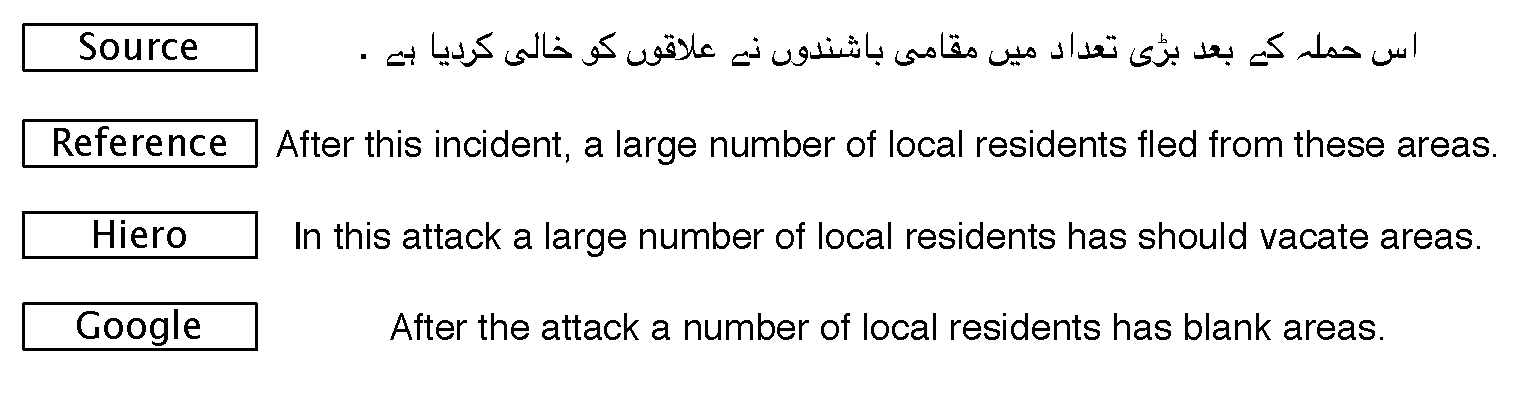
\includegraphics[scale=0.55]{urdu_example_translation.pdf}
\caption{An example Urdu $\rightarrow$ English translation show outputs from both a state-of-the-art Hiero translation model, and Google's translation service.}
\label{fig:intro_urdu_example}
\end{figure}
Figure \ref{fig:intro_urdu_example} shows the current state-of-the-art for translating an Urdu sentence into English.
While a considerable portion of the content of the input Urdu sentence is translated, the end result is still far from being acceptable for an end user. 
%\begin{figure}
%  \centering \includegraphics[scale=1.3]{intro_slides/WhoWroteThisLetter.pdf}
%\caption{The level of structural divergence varies depending on the language pair in question.}
%\label{fig:intro_translation_divergence}
%\end{figure}
Many of the issues faced by SMT systems can be attributed to structural divergence between the languages being translated.
While many researchers are tackling these issues, most proposed solutions are limited by focusing on more expressive models of translation rather than addressing the issue of how, and what, translation units are learnt a priori.


\begin{table}[t]
\centering
  \begin{tabular}{l|rr}
    \hline
    Language & Words &  Domain \\ \hline
    English & 4.5M& Financial news \\
    Chinese & 0.5M & Broadcasting news \\ 
    Arabic &  300K (1M planned)  &  News  \\
    Korean & 54K  & Military \\ \hline
  \end{tabular}
\caption{Major treebanks: data size and domain.}
\label{tab:intro_treebanks}
\end{table}
%\begin{figure}
%  \centering 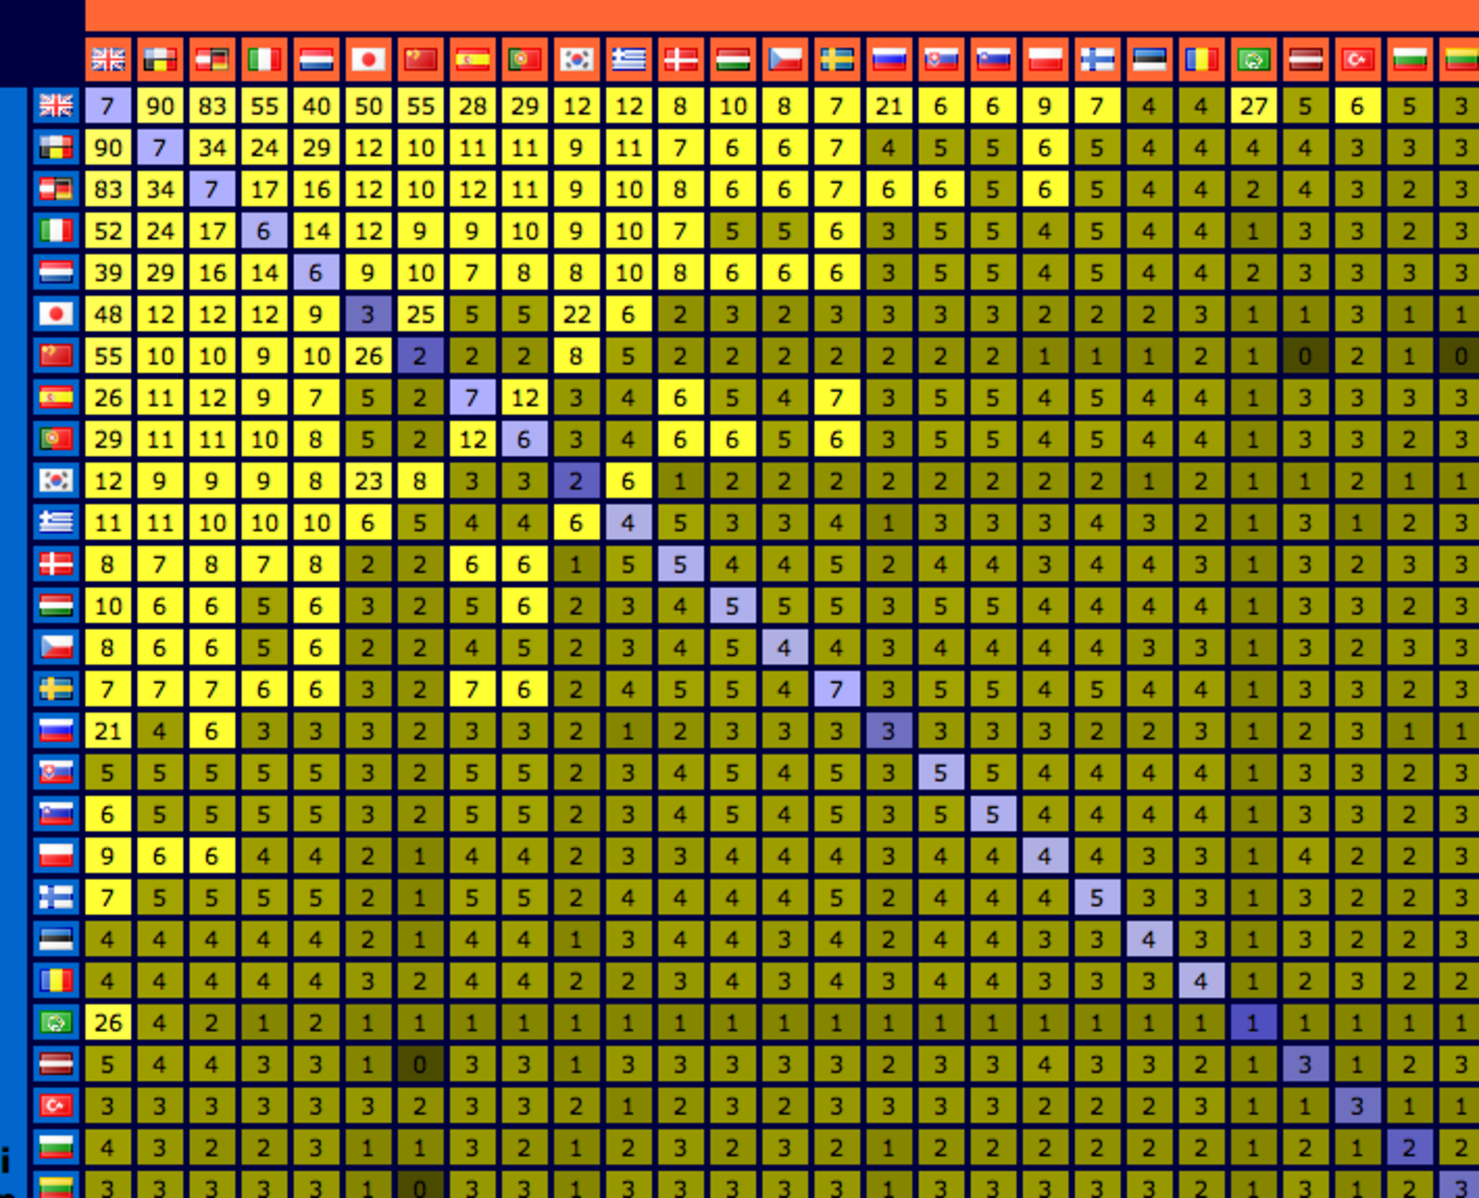
\includegraphics[scale=0.3]{intro_slides/resource_matrix.pdf}
%\caption{A matrix of the number of parrallel words available for various language pairs.}
%\label{fig:intro_parallel_words_matrix}
%\end{figure}

\begin{figure}[t]
  \centering
  \subfigure{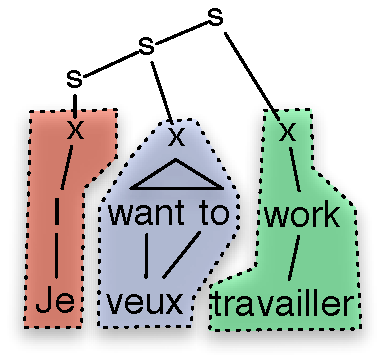
\includegraphics[scale=0.5]{intro_slides/JeVeuxTravailler-Hiero.pdf}}
  \subfigure{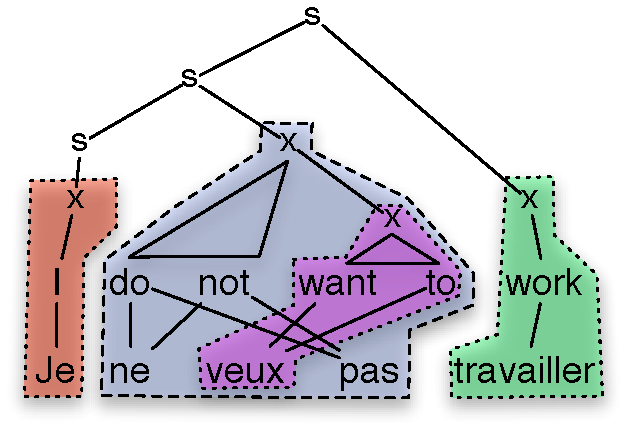
\includegraphics[scale=0.5]{intro_slides/JeNeVeuxPasTravailler-Hiero.pdf}}
\caption{Example derivations using the Hiero grammar extraction heuristics \cite{chiang07hierarchical}.}
\label{fig:intro_hiero}
\end{figure}

\begin{figure}[t]
  \centering
  \subfigure{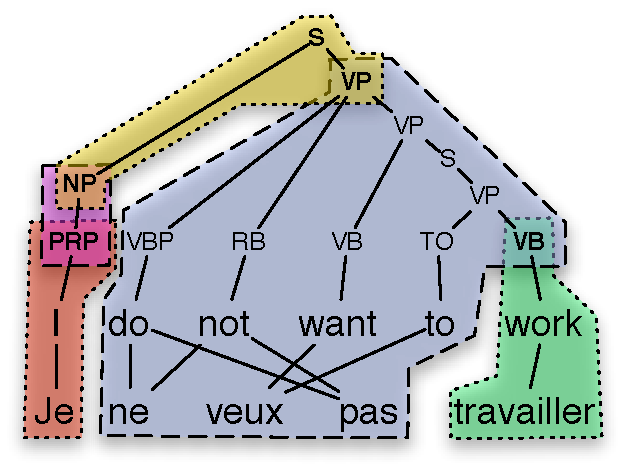
\includegraphics[scale=0.5]{intro_slides/JeNeVeuxPasTravailler-tsg.pdf}}
  \subfigure{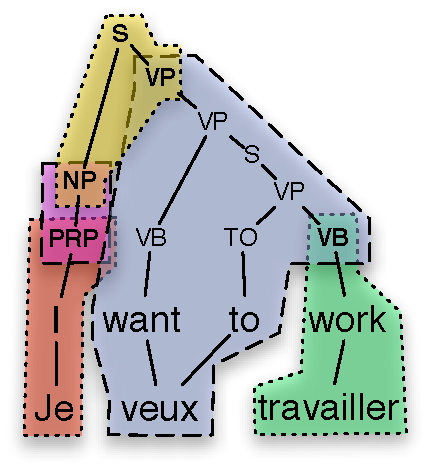
\includegraphics[scale=0.5]{intro_slides/JeVeuxTravailler-tsg.pdf}}
\caption{Example derivations for a Tree Substitution Grammar derived from a parallel corpus parsed with a supervised parser.}
\label{fig:intro_tsg}
\end{figure}

Models which have been most successful for translating between structurally divergent language pairs have been based on synchronous grammars. 
A critical component of these translation models is their {\emph grammar} which encodes translational equivalence and licenses reordering between tokens in the source and target languages. 
There is considerable scope for improving beyond current techniques for automatically acquiring synchronous grammars from bilingual corpora, which seek to find either extremely simple grammars with only one non-terminal or else rely on treebank-trained parsers.
The advantage of using a simple grammar is that no extra annotated linguistic resources are required beyond the parallel corpus.
However these simple grammars are incapable of representing the substitutability of a constituent.
Figure \ref{fig:intro_hiero} displays a synchronous derivation in such a simple grammar.
Richer grammars induced from a parallel corpus annotated with syntax trees overcome the limitations of the simple grammars and provide a far more powerful representation of language structure. 
Figure \ref{fig:intro_tsg} shows a synchronous derivation in for a grammar extracted parallel corpus parsed on the English side.
The limitation of this approach is that the reliance on supervised parses restricts the systems' portability to new target languages (effectively limiting us to translating into/out of English) while enforcing a restrictive notion of linguistic constituency. 
Figure \ref{fig:intro_parallel_words_matrix} shows the number of words in the treebanks available for the most well resourced languages. 
As the performance of supervised parsers is heavily dependent on the amount of training data available, clearly we can expect poorer results when building translation models based upon then for languages other than English.
A further, but more subtle, limitation of these models is the assumption that the particular brand of linguistic structure assigned by a parser (usually a form of phrase structure grammar learnt from the Penn. Treebank) is predominantly isomorphic to that of the input language; an assumption which is rarely true for distantly related language pairs, or even closely related ones.



Clearly there is a need for research into the unsupervised induction of synchronous grammar based translation models.
Previous research has focussed on structured learning approaches requiring costly global inference over translation pair derivations, limiting the ability of these models to be scaled to large datasets \cite{blunsom09bscfg}.
In this workshop we adopted a pragmatic approach of embracing existing algorithms for inducing unlabelled SCFGs (e.g. the popular Hiero model \cite{chiang07hierarchical}), and then used state-of-the-art probabilistic models to independently learn syntactic classes for translation rules in the grammar.
We structured the workshop into three parallel but interdependent streams:

\begin{figure}
  \centering
  \subfigure{\includegraphics[scale=0.5]{intro_slides/JeNeVeuxPasTravailler-hiero-labelled.pdf}}
\caption{Example derivation using the Hiero grammar extraction heuristics where non-terminals have been clustered into unsupervised syntactic categories denoted by $X?$.}
\label{fig:intro_labelled_hiero}
\end{figure}


\paragraph{1) Unsupervised induction of labelled SCFGs}
Inspired by work in monolingual PCFG learning, we have investigated generative models which describe the production of phrase translations in terms of sequences of tokens (or word classes) and their observed contexts.
We simplify the grammar induction problem to first clustering monolingual phrases based upon their distribution over contexts (preceding and following words), and then intersecting these labelled phrases with the Hiero \cite{chiang07hierarchical} SCFG rule extraction heuristics. 
The end result are grammars that produce derivations like that in Figure \ref{fig:intro_labelled_hiero}, where the labels are the unsupervised clusters induced by our context based induction algorithm.

We explored two approaches to the clustering of phrases.
The first was inspired by research in Topic Modelling, in particular Latent Dirichlet Allocation (LDA).
We formulated a model in which each phrase type maintains a distribution over labels, and each context a phrase appears in is generated by first choosing a label, and then generating the context from this labels distribution over contexts.
We extended the basic LDA model to incorporate hierarchical Pitman Yor distributions on the two generating components of the model.
In the second approach we optimised the same model as describe above, but in instead of using non-parametric Bayesian approach to encouraging sparsity in the model, we used the direct Posterior Regularisation technique of \cite{someone}. 

The labelled SCFGs produced by these algorithms generate a subset of the translations licensed by the original Hiero grammars.
While we hope that this restriction guides the model to more acceptable translations, with the inevitable noise present in all automatically induced translation models it is advantageous to allow our models to degrade gracefully to less restrictive grammars.
As such we also explored hierarchical cascades of grammars, each of which was induced with a different number of labels, allowing the translation model to switch between these while incurring a penalty for doing so.

This work on inducing labels for SCFGs formed the core component of the workshop and the base for the following work exploiting these labellings. 
By the conclusion of the workshop we were able to demonstrate that applying these induction techniques leads to improved translations for both Chinese$\rightarrow$English and Urdu$\rightarrow$ translation systems.
Chapter \ref{chap:grammar_induction} describes this work.

\paragraph{2) Decoding with labelled SCFGs}
The second major component of the workshop involved the investigation of improved decoding algorithms for the type of labelled SCFG produced by our induction methods.
Decoding complexity scales quadratically with the number of labels in the grammar.
As such inducing grammars with more than one label significantly increases the time and resources required for decoding.
We explored a number of avenues for reducing this computational burden, including the early pruning items from the search space before language model integration, and coarse-to-fine techniques in which decoding is performed with grammars with progressively more labels and pruning at each step.
We were able to show that each of these techniques could lead to faster decoding without compromising translations performance.
Chapter \ref{chap:decoding} describes this work.

\paragraph{3) Discriminative training labelled SCFG translation models}
Chapter \ref{chap:training} describes this work.

The remainder of this introductory chapter provides a formal definition of SCFGs and describes the language pairs that we experimented with.

\section{Synchronous context free grammar} \label{sec:scfg}

A synchronous context free grammar (SCFG, \cite{lewis68scfg}) generalizes context-free grammars to generate strings concurrently in two (or more) languages. A string pair is generated by applying a series of paired rewrite rules of the form, $X \rightarrow \langle \mathbf{e}, \mathbf{f}, \mathbf{a} \rangle$, where $X$ is a non-terminal, $\mathbf{e}$ and $\mathbf{f}$ are strings of terminals and non-terminals and $\mathbf{a}$ specifies a one-to-one alignment between non-terminals in $\mathbf{e}$ and $\mathbf{f}$.
In the context of SMT, by assigning the source and target languages to the respective sides of a probabilistic SCFG it is possible to describe translation as the process of parsing the source sentence, which induces a parallel tree structure and translation in the target language \cite{chiang07hierarchical}.  
Terminal are rewritten as pairs of strings of terminal symbols in the source and target languages.  Additionally, one side of a terminal expansion may be the special symbol $\epsilon$, which indicates a null alignment which permits arbitrary insertions and deletions.
Figure \ref{fig:scfg} shows an example derivation for Japanese to English translation using an SCFG.

\begin{figure}Grammar fragment:
\begin{eqnarray*}
\label{rule:discont}X & \rightarrow & \langle \nt{X}{1}\ \nt{X}{2}\ \nt{X}{3},\ \nt{X}{1}\ \nt{X}{3}\ \nt{X}{2} \rangle  \\
X & \rightarrow & \langle \textrm{\emph{John-ga}},\ \textrm{\emph{John}} \rangle  \\
X & \rightarrow & \langle \textrm{\emph{ringo-o}},\ \textrm{\emph{an apple}} \rangle  \\
X & \rightarrow & \langle \textrm{\emph{tabeta}},\ \textrm{\emph{ate}} \rangle
\end{eqnarray*}
Sample derivation:
\begin{eqnarray*}
\label{derivationt}
& &\langle \nt{S}{1},\nt{S}{1} \rangle \Rightarrow \langle \nt{X}{2},\ \nt{X}{2} \rangle \\
 & \Rightarrow&  \langle \nt{X}{3}\ \nt{X}{4}\ \nt{X}{5},\ \nt{X}{3}\ \nt{X}{5}\ \nt{X}{4} \rangle  \\
 & \Rightarrow &\langle \textrm{\emph{John-ga}}\ \nt{X}{4}\ \nt{X}{5},\ \textrm{\emph{John}}\ \nt{X}{5}\ \nt{X}{4} \rangle \\
 & \Rightarrow &\langle \textrm{\emph{John-ga}}\ \textrm{\emph{ringo-o}}\ \nt{X}{5},\ \textrm{\emph{John}}\ \nt{X}{5}\ \textrm{\emph{an apple}} \rangle \\
 & \Rightarrow &\langle \textrm{\emph{John-ga ringo-o tabeta}},\ \textrm{\emph{John ate an apple}} \rangle
\end{eqnarray*}
\caption{A fragment of an SCFG with a ternary non-terminal expansion and three terminal rules.}
\label{fig:scfg}
\end{figure}

The generative story is as follows. 
In the beginning was the grammar, in which we allow  two types of rules: {\emph non-terminal} and {\emph terminal} expansions. 
The former rewrites a non-terminal symbol as a string of two or three non-terminals along with an alignment $\mathbf{a}$, specifying the corresponding ordering of the child trees in the source and target language. 
Terminal expansion rewrite a non-terminal as a pair of terminal n-grams, where either but not both may be empty. 
Given a grammar, each sentence is generated as follows, starting with the distinguished root non-terminal, $S$. 
Rewrite each frontier non-terminal, $c$, using a rule chosen from our grammar expanding $c$. 
Repeat until there are no remaining frontier non-terminals. 
The sentences in both languages can then be read off the leaves, using the rules' alignments to find the right ordering. 


